% Homework 4 - CS350
% Russell Miller Winter 2011

\documentclass{article}
\usepackage{anysize}
\usepackage{fullpage}
\usepackage{cancel}
\usepackage{graphicx}

\marginsize{2cm}{2cm}{2cm}{2cm}

\title{CS350 Homework 4}
\author{Russell Miller}
\date{\today}

\begin{document}

\maketitle

\section*{24.3-6}
\begin{verbatim}
MOST-RELIABLE-PATH(G, source)
1  mark each vertex as distance infinity
2  mark each vertex's previous vertex as undefined
3  mark the source's distance as 0
4  put all of the vertices in a Queue
5  while the Queue is not empty
6    find the vertex u with the least distance
7    if that vertex is the target
8      create a new sequence S
9      while previous vertex of u is defined
10       add u at the beginning of S
11       continue to u's previous vertex
12     remove that vertex from the Queue
13   for each neighbor v of that vertex
14     add the negative logs of u and (u,v)
15     if the sum is less than the current value of v's distance
16       set v's distance to that sum
17       set v's previous vertex to u
\end{verbatim}

\section*{15.2-1}
For this problem I wrote the Matrix-Chain-Order and Print-Optimal-
Parens functions in Python, using the pseudocode from the textbook.
My code is below:
\begin{verbatim}
import sys

def main():
    # dimensions of each matrix
    a = [5,10,3,12,5,50,6]
    m,s = matrix_chain_order(a)
    for line in m:
        print(line)
    for line in s:
        print(line)
    print_opt_parens(s,1,6)
    sys.stdout.write('\n')

\end{verbatim}
\pagebreak
\begin{verbatim}
def matrix_chain_order(p):
    n = len(p) - 1
    m = []
    s = []
    for i in range(n):
        m.append([])
        s.append([])
        for j in range(n):
            m[i].append(0)
            s[i].append(0)
    for l in range(2,n+1):
        for i in range(1,n-l+2):
            j = i + l - 1
            m[i-1][j-1] = 9999
            for k in range(i,j):
                q = m[i-1][k-1] + m[k][j-1] + p[i-1]*p[k]*p[j]
                if q < m[i-1][j-1]:
                    m[i-1][j-1] = q
                    s[i-1][j-1] = k            
    return m,s

def print_opt_parens(s,i,j):
    if i == j:
        sys.stdout.write("A_" + str(i) + " ")
    else:
        sys.stdout.write("(")
        print_opt_parens(s,i,s[i-1][j-1])
        print_opt_parens(s,s[i-1][j-1] + 1, j)
        sys.stdout.write(")")

if __name__=="__main__":
    main()
\end{verbatim}
The output of the program is:
\begin{verbatim}
[0, 150, 330, 405, 1655, 2010]
[0, 0, 360, 330, 2430, 1950]
[0, 0, 0, 180, 930, 1770]
[0, 0, 0, 0, 3000, 1860]
[0, 0, 0, 0, 0, 1500]
[0, 0, 0, 0, 0, 0]
[0, 1, 2, 2, 4, 2]
[0, 0, 2, 2, 2, 2]
[0, 0, 0, 3, 4, 4]
[0, 0, 0, 0, 4, 4]
[0, 0, 0, 0, 0, 5]
[0, 0, 0, 0, 0, 0]
((A_1 A_2 )((A_3 A_4 )(A_5 A_6 )))
\end{verbatim}

\section*{16.2-2}
For this algorithm, I'm going to go with a few assumptions.\\
First of all, W is a multiple of 100. Also, each item is a value
n * 100 for values of n up to and including n * 100 = W.\\
This builds a table like the one in class, and returns the very
last value of the table.\\

\pagebreak

\begin{verbatim}
KNAPSACK(W, n)
1  create new table K [1..n , 100..W]
2  set each value of column 1 to 100
3  set each value of row 100 to 100
4  for i = 2 to n
5    for j = 200 to W
6      max = -1
7      current_sum = 0
8      if i*100 <= j
9        current_sum = put item i*100
10       if j-i*100 > 0
11         current_sum += K[i-1][j-i*100]
12       endif
13       if current_sum > max
14         max = current_sum
15       endif
16     else if K[i-1][j] > max
17       max = K[i-1][j]
18     endif
19   endfor
20 endfor
21 return K[n][W]
\end{verbatim}

\section*{16.3-3}
I used the algorithm in the book to build a tree, where the edges are the encodings.\\
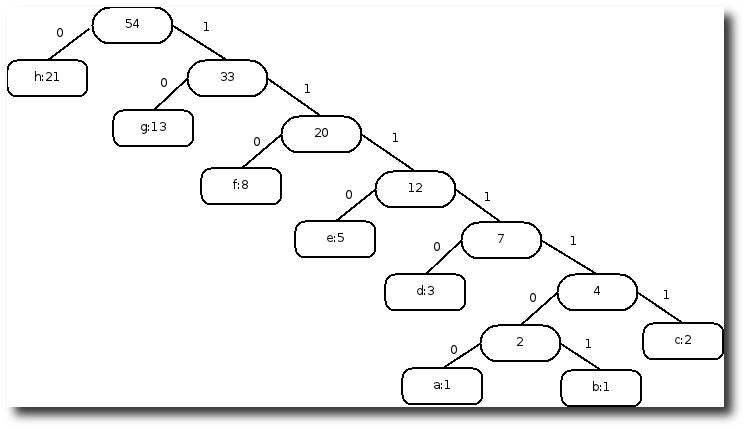
\includegraphics[scale=.5]{3-2.png}
\\So the encodings would be:
\begin{verbatim}
a: 1111100
b: 1111101
c: 111111
d: 11110
e: 1110
f: 110
g: 10
h: 0
\end{verbatim}
The algorithm is able to handle any value of n. With this sequence of values, however,
a very inefficient encoding is created.\\\\
\textbf{16.3-9} - \emph{I am not going to attempt this one.}
\end{document}
